\documentclass[10pt]{article}
\usepackage[polish]{babel}
\usepackage[utf8]{inputenc}
\usepackage[T1]{fontenc}
\usepackage{graphicx}
\usepackage[export]{adjustbox}
\graphicspath{ {./images/} }
\usepackage{amsmath}
\usepackage{amsfonts}
\usepackage{amssymb}
\usepackage[version=4]{mhchem}
\usepackage{stmaryrd}
\usepackage{multirow}

\title{PRÓBNY EGZAMIN MATURALNY Z NOWĄ ERĄ MATEMATYKA - POZIOM ROZSZERZONY }

\author{}
\date{}


\begin{document}
\maketitle
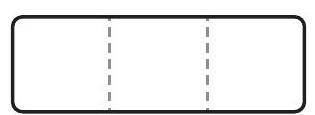
\includegraphics[max width=\textwidth, center]{2024_11_21_50d2fc5b1407ca7ef55bg-01}\\
symbol klasy\\
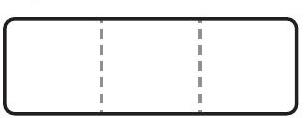
\includegraphics[max width=\textwidth, center]{2024_11_21_50d2fc5b1407ca7ef55bg-01(1)}\\
symbol zdającego

\section*{Instrukcja dla zdającego}
\begin{enumerate}
  \item Sprawdź, czy arkusz egzaminacyjny zawiera 22 strony (zadania 1-16). Ewentualny brak stron zgłoś nauczycielowi nadzorującemu egzamin.
  \item Rozwiązania zadań i odpowiedzi zapisz w miejscu na to przeznaczonym.
  \item Pamiętaj, że pominięcie argumentacji lub istotnych obliczeń w rozwiązaniu zadań otwartych może spowodować, że za to rozwiązanie nie otrzymasz pełnej liczby punktów.
  \item Pisz czytelnie. Używaj długopisu/pióra tylko z czarnym tuszem/atramentem.
  \item Nie używaj korektora, a błędne zapisy wyraźnie przekreśl.
  \item Pamiętaj, że zapisy w brudnopisie nie będą oceniane.
  \item Podczas egzaminu możesz korzystać z zestawu wzorów matematycznych, cyrkla i linijki oraz kalkulatora prostego.
  \item Na tej stronie wpisz swój kod.
  \item Nie wpisuj żadnych znaków w części przeznaczonej dla osoby sprawdzającej.
\end{enumerate}

\section*{Powodzenia!}
\section*{\(\square\) \\
 dysleksja}
STYCZEŃ 2022

Czas pracy:\\
180 minut

Liczba punktów\\
do uzyskania: 50

W zadaniach 1.-4. wybierz i zaznacz poprawną odpowiedź.

\section*{Zadanie 1. (0-1)}
Rozwiązaniem równania \(\sqrt{\log x}=\log \sqrt{x}\)\\
A. jest tylko liczba 1.\\
B. jest między innymi liczba 10000.\\
C. nie może być żadna liczba większa od 1.\\
D. nie może być żadna liczba wymierna.

\section*{Zadanie 2. (0-1)}
Jedynymi miejscami zerowymi funkcji \(f\), określonej dla każdej liczby rzeczywistej \(x\), są liczby 0 oraz 2022. Miejscami zerowymi funkcji \(g(x)=f(2022 \cdot x)\) są liczby\\
A. 0 i \(2022^{2}\).\\
B. 0 i 1 .\\
C. 2022 i \(2022^{2}\).\\
D. 1 i 2022 .

\section*{Zadanie 3. (0-1)}
Funkcja \(f\) jest określona wzorem \(f(x)=(x+1)(x-2)(x-3)+4\) dla każdej liczby rzeczywistej \(x\). Współczynnik kierunkowy a stycznej do wykresu tej funkcji w punkcie \(A=(2,4)\) spełnia warunek\\
A. \(a<0\).\\
B. \(0 \leqslant a<1\).\\
C. \(a=1\).\\
D. \(a>1\).

\section*{Zadanie 4. (0-1)}
Liczba \(4 \cos 75^{\circ} \cdot \cos 15^{\circ}\) jest równa\\
A. \(\frac{1}{2}\).\\
B. \(\frac{\sqrt{2}}{2}\).\\
C. \(\frac{\sqrt{3}}{2}\).\\
D. 1 .

\section*{BRUDNOPIS (nie podlega ocenie)}
\begin{center}

\includegraphics[max width=\textwidth]{2024_11_21_50d2fc5b1407ca7ef55bg-03}
\end{center}

\begin{center}
\begin{tabular}{|l|l|c|c|c|c|}
\hline
\multirow{2}{*}{\begin{tabular}{c}
Wypełnia \\
sprawdzający \\
\end{tabular}} & Nr zadania & 1 & 2 & 3 & 4 \\
\cline { 2 - 6 }
 & Maks. liczba pkt & 1 & 1 & 1 & 1 \\
\cline { 2 - 6 }
 & Uzyskana liczba pkt &  &  &  &  \\
\hline
\end{tabular}
\end{center}

Zadanie 5. (0-2)\\
Rozwiąż równanie \(1+\frac{1}{x-1}+\left(\frac{1}{x-1}\right)^{2}+\left(\frac{1}{x-1}\right)^{3}+\ldots=\frac{9}{2}\), którego lewa strona jest sumą wszystkich wyrazów nieskończonego ciągu geometrycznego.\\
W kratki poniżej wpisz kolejno - od lewej do prawej - cyfrę jedności oraz pierwszą i drugą cyfrę po przecinku nieskończonego rozwinięcia dziesiętnego otrzymanego wyniku.\\
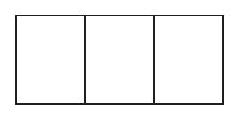
\includegraphics[max width=\textwidth, center]{2024_11_21_50d2fc5b1407ca7ef55bg-04}

\begin{center}
\begin{tabular}{|c|c|c|c|c|c|c|c|c|c|c|c|c|c|c|c|c|c|c|c|c|c|c|c|}
\hline
 &  &  &  &  &  &  &  &  &  &  &  &  &  &  &  &  &  &  &  &  &  &  &  \\
\hline
 &  &  &  &  &  &  &  &  &  &  &  &  &  &  &  &  &  &  &  &  &  &  &  \\
\hline
 &  &  &  &  &  &  &  &  &  &  &  &  &  &  &  &  &  &  &  &  &  &  &  \\
\hline
 &  &  &  &  &  &  &  &  &  &  &  &  &  &  &  &  &  &  &  &  &  &  &  \\
\hline
 &  &  &  &  &  &  &  &  &  &  &  &  &  &  &  &  &  &  &  &  &  &  &  \\
\hline
 &  &  &  &  &  &  &  &  &  &  &  &  &  &  &  &  &  &  &  &  &  &  &  \\
\hline
 &  &  &  &  &  &  &  &  &  &  &  &  &  &  &  &  &  &  &  &  &  &  &  \\
\hline
 &  &  &  &  &  &  &  &  &  &  &  &  &  &  &  &  &  &  &  &  &  &  &  \\
\hline
 &  &  &  &  &  &  &  &  &  &  &  &  &  &  &  &  &  &  &  &  &  &  &  \\
\hline
 &  &  &  &  &  &  &  &  &  &  &  &  &  &  &  &  &  &  &  &  &  &  &  \\
\hline
 &  &  &  &  &  &  &  &  &  &  &  &  &  &  &  &  &  &  &  &  &  &  &  \\
\hline
 &  &  &  &  &  &  &  &  &  &  &  &  &  &  &  &  &  &  &  &  &  &  &  \\
\hline
 &  &  &  &  &  &  &  &  &  &  &  &  &  &  &  &  &  &  &  &  &  &  &  \\
\hline
 &  &  &  &  &  &  &  &  &  &  &  &  &  &  &  &  &  &  &  &  &  &  &  \\
\hline
 &  &  &  &  &  &  &  &  &  &  &  &  &  &  &  &  &  &  &  &  &  &  &  \\
\hline
 &  &  &  &  &  &  &  &  &  &  &  &  &  &  &  &  &  &  &  &  &  &  &  \\
\hline
 &  &  &  &  &  &  &  &  &  &  &  &  &  &  &  &  &  &  &  &  &  &  &  \\
\hline
 &  &  &  &  &  &  &  &  &  &  &  &  &  &  &  &  &  &  &  &  &  &  &  \\
\hline
 &  &  &  &  &  &  &  &  &  &  &  &  &  &  &  &  &  &  &  &  &  &  &  \\
\hline
 &  &  &  &  &  &  &  &  &  &  &  &  &  &  &  &  &  &  &  &  &  &  &  \\
\hline
 &  &  &  &  &  &  &  &  &  &  &  &  &  &  &  &  &  &  &  &  &  &  &  \\
\hline
 &  &  &  &  &  &  &  &  &  &  &  &  &  &  &  &  &  &  &  &  &  &  &  \\
\hline
 &  &  &  &  &  &  &  &  &  &  &  &  &  &  &  &  &  &  &  &  &  &  &  \\
\hline
 &  &  &  &  &  &  &  &  &  &  &  &  &  &  &  &  &  &  &  &  &  &  &  \\
\hline
 &  &  &  &  &  &  &  &  &  &  &  &  &  &  &  &  &  &  &  &  &  &  &  \\
\hline
 &  &  &  &  &  &  &  &  &  &  &  &  &  &  &  &  &  &  &  &  &  &  &  \\
\hline
 &  &  &  &  &  &  &  &  &  &  &  &  &  &  &  &  &  &  &  &  &  &  &  \\
\hline
 &  &  &  &  &  &  &  &  &  &  &  &  &  &  &  &  &  &  &  &  &  &  &  \\
\hline
 &  &  &  &  &  &  &  &  &  &  &  &  &  &  &  &  &  &  &  &  &  &  &  \\
\hline
 &  &  &  &  &  &  &  &  &  &  &  &  &  &  &  &  &  &  &  &  &  &  &  \\
\hline
 &  &  &  &  &  &  &  &  &  &  &  &  &  &  &  &  &  &  &  &  &  &  &  \\
\hline
 &  &  &  &  &  &  &  &  &  &  &  &  &  &  &  &  &  &  &  &  &  &  &  \\
\hline
 &  &  &  &  &  &  &  &  &  &  &  &  &  &  &  &  &  &  &  &  &  &  &  \\
\hline
 &  &  &  &  &  &  &  &  &  &  &  &  &  &  &  &  &  &  &  &  &  &  &  \\
\hline
 &  &  &  &  &  &  &  &  &  &  &  &  &  &  &  &  &  &  &  &  &  &  &  \\
\hline
 &  &  &  &  &  &  &  &  &  &  &  &  &  &  &  &  &  &  &  &  &  &  &  \\
\hline
 &  &  &  &  &  &  &  &  &  &  &  &  &  &  &  &  &  &  &  &  &  &  &  \\
\hline
 &  &  &  &  &  &  &  &  &  &  &  &  &  &  &  &  &  &  &  &  &  &  &  \\
\hline
\end{tabular}
\end{center}

Zadanie 6. (0-2)\\
Oblicz \(\lim _{n \rightarrow+\infty}\left(\frac{6 n^{2}+1}{3 n-1}-\frac{4 n^{2}-3}{2 n+1}\right)\).

\begin{center}
\begin{tabular}{|c|c|c|c|c|c|c|c|c|c|c|c|c|c|c|c|c|c|c|c|c|c|c|c|c|c|c|c|c|c|}
\hline
 &  &  &  &  &  &  &  &  &  &  &  &  &  &  &  &  &  &  &  &  &  &  &  &  &  &  &  &  &  \\
\hline
 &  &  &  &  &  &  &  &  &  &  &  &  &  &  &  &  &  &  &  &  &  &  &  &  &  &  &  &  &  \\
\hline
 &  &  &  &  &  &  &  &  &  &  &  &  &  &  &  &  &  &  &  &  &  &  &  &  &  &  &  &  &  \\
\hline
 &  &  &  &  &  &  &  &  &  &  &  &  &  &  &  &  &  &  &  &  &  &  &  &  &  &  &  &  &  \\
\hline
 &  &  &  &  &  &  &  &  &  &  &  &  &  &  &  &  &  &  &  &  &  &  &  &  &  &  &  &  &  \\
\hline
 &  &  &  &  &  &  &  &  &  &  &  &  &  &  &  &  &  &  &  &  &  &  &  &  &  &  &  &  &  \\
\hline
 &  &  &  &  &  &  &  &  &  &  &  &  &  &  &  &  &  &  &  &  &  &  &  &  &  &  &  &  &  \\
\hline
 &  &  &  &  &  &  &  &  &  &  &  &  &  &  &  &  &  &  &  &  &  &  &  &  &  &  &  &  &  \\
\hline
 &  &  &  &  &  &  &  &  &  &  &  &  &  &  &  &  &  &  &  &  &  &  &  &  &  &  &  &  &  \\
\hline
 &  &  &  &  &  &  &  &  &  &  &  &  &  &  &  &  &  &  &  &  &  &  &  &  &  &  &  &  &  \\
\hline
 &  &  &  &  &  &  &  &  &  &  &  &  &  &  &  &  &  &  &  &  &  &  &  &  &  &  &  &  &  \\
\hline
 &  &  &  &  &  &  &  &  &  &  &  &  &  &  &  &  &  &  &  &  &  &  &  &  &  &  &  &  &  \\
\hline
 &  &  &  &  &  &  &  &  &  &  &  &  &  &  &  &  &  &  &  &  &  &  &  &  &  &  &  &  &  \\
\hline
 &  &  &  &  &  &  &  &  &  &  &  &  &  &  &  &  &  &  &  &  &  &  &  &  &  &  &  &  &  \\
\hline
 &  &  &  &  &  &  &  &  &  &  &  &  &  &  &  &  &  &  &  &  &  &  &  &  &  &  &  &  &  \\
\hline
 &  &  &  &  &  &  &  &  &  &  &  &  &  &  &  &  &  &  &  &  &  &  &  &  &  &  &  &  &  \\
\hline
 &  &  &  &  &  &  &  &  &  &  &  &  &  &  &  &  &  &  &  &  &  &  &  &  &  &  &  &  &  \\
\hline
 &  &  &  &  &  &  &  &  &  &  &  &  &  &  &  &  &  &  &  &  &  &  &  &  &  &  &  &  &  \\
\hline
 &  &  &  &  &  &  &  &  &  &  &  &  &  &  &  &  &  &  &  &  &  &  &  &  &  &  &  &  &  \\
\hline
 &  &  &  &  &  &  &  &  &  &  &  &  &  &  &  &  &  &  &  &  &  &  &  &  &  &  &  &  &  \\
\hline
 &  &  &  &  &  &  &  &  &  &  &  &  &  &  &  &  &  &  &  &  &  &  &  &  &  &  &  &  &  \\
\hline
 &  &  &  &  &  &  &  &  &  &  &  &  &  &  &  &  &  &  &  &  &  &  &  &  &  &  &  &  &  \\
\hline
 &  &  &  &  &  &  &  &  &  &  &  &  &  &  &  &  &  &  &  &  &  &  &  &  &  &  &  &  &  \\
\hline
 &  &  &  &  &  &  &  &  &  &  &  &  &  &  &  &  &  &  &  &  &  &  &  &  &  &  &  &  &  \\
\hline
 &  &  &  &  &  &  &  &  &  &  &  &  &  &  &  &  &  &  &  &  &  &  &  &  &  &  &  &  &  \\
\hline
 &  &  &  &  &  &  &  &  &  &  &  &  &  &  &  &  &  &  &  &  &  &  &  &  &  &  &  &  &  \\
\hline
 &  &  &  &  &  &  &  &  &  &  &  &  &  &  &  &  &  &  &  &  &  &  &  &  &  &  &  &  &  \\
\hline
 &  &  &  &  &  &  &  &  &  &  &  &  &  &  &  &  &  &  &  &  &  &  &  &  &  &  &  &  &  \\
\hline
 &  &  &  &  &  &  &  &  &  &  &  &  &  &  &  &  &  &  &  &  &  &  &  &  &  &  &  &  &  \\
\hline
 &  &  &  &  &  &  &  &  &  &  &  &  &  &  &  &  &  &  &  &  &  &  &  &  &  &  &  &  &  \\
\hline
 &  &  &  &  &  &  &  &  &  &  &  &  &  &  &  &  &  &  &  &  &  &  &  &  &  &  &  &  &  \\
\hline
 &  &  &  &  &  &  &  &  &  &  &  &  &  &  &  &  &  &  &  &  &  &  &  &  &  &  &  &  &  \\
\hline
 &  &  &  &  &  &  &  &  &  &  &  &  &  &  &  &  &  &  &  &  &  &  &  &  &  &  &  &  &  \\
\hline
 &  &  &  &  &  &  &  &  &  &  &  &  &  &  &  &  &  &  &  &  &  &  &  &  &  &  &  &  &  \\
\hline
 &  &  &  &  &  &  &  &  &  &  &  &  &  &  &  &  &  &  &  &  &  &  &  &  &  &  &  &  &  \\
\hline
 &  &  &  &  &  &  &  &  &  &  &  &  &  &  &  &  &  &  &  &  &  &  &  &  &  &  &  &  &  \\
\hline
\end{tabular}
\end{center}

Odpowiedź:

\begin{center}
\begin{tabular}{|l|l|c|c|}
\hline
\multirow{2}{*}{\begin{tabular}{c}
Wypełnia \\
sprawdzający \\
\end{tabular}} & Nr zadania & 5 & 6 \\
\cline { 2 - 4 }
 & Maks. liczba pkt & 2 & 2 \\
\cline { 2 - 4 }
 & Uzyskana liczba pkt &  &  \\
\hline
\end{tabular}
\end{center}

Zadanie 7. (0-2)\\
Funkcja \(f\) jest określona wzorem \(f(x)=\frac{1}{x-1}+3\) dla każdej liczby rzeczywistej \(x \neq 1\). Wyznacz wszystkie punkty leżące na wykresie funkcji \(f\), których obie współrzędne są liczbami całkowitymi.\\

\includegraphics[max width=\textwidth, center]{2024_11_21_50d2fc5b1407ca7ef55bg-06}

Odpowiedź:

Zadanie 8. (0-3)\\
Wykaż, że dla każdej dodatniej liczby rzeczywistej \(x\) i każdej liczby rzeczywistej \(y>1\) prawdziwa jest nierówność

\[
x^{2}+y^{2}>x(y+1)
\]

\begin{center}

\includegraphics[max width=\textwidth]{2024_11_21_50d2fc5b1407ca7ef55bg-07}
\end{center}

\begin{center}
\begin{tabular}{|l|l|c|c|}
\hline
\multirow{3}{*}{\begin{tabular}{c}
Wypełnia \\
sprawdzający \\
\end{tabular}} & Nr zadania & 7 & 8 \\
\cline { 2 - 4 }
 & Maks. liczba pkt & 2 & 3 \\
\cline { 2 - 4 }
 & Uzyskana liczba pkt &  &  \\
\hline
\end{tabular}
\end{center}

Zadanie 9. (0-3)\\
Rozwiąż równanie \(8 \sin ^{3} x+4 \cos ^{2} x=1+6 \sin x\).\\

\includegraphics[max width=\textwidth, center]{2024_11_21_50d2fc5b1407ca7ef55bg-08}

Odpowiedź:

Zadanie 10. (0-4)\\
Spośród zaznaczonych 16 punktów sieci kwadratowej (zobacz rysunek) wybrano losowo trzy różne punkty. Oblicz prawdopodobieństwo zdarzenia polegającego na tym, że wylosowane punkty są wierzchołkami trójkąta. Wynik podaj w postaci ułamka nieskracalnego.\\
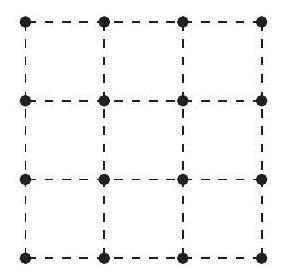
\includegraphics[max width=\textwidth, center]{2024_11_21_50d2fc5b1407ca7ef55bg-09}

\begin{center}
\begin{tabular}{|c|c|c|c|c|c|c|c|c|c|c|c|c|c|c|c|c|c|c|c|c|c|c|c|c|c|c|c|c|c|}
\hline
 &  &  &  &  &  &  &  &  &  &  &  &  &  &  &  &  &  &  &  &  &  &  &  &  &  &  &  &  &  \\
\hline
 &  &  &  &  &  &  &  &  &  &  &  &  &  &  &  &  &  &  &  &  &  &  &  &  &  &  &  &  &  \\
\hline
 &  &  &  &  &  &  &  &  &  &  &  &  &  &  &  &  &  &  &  &  &  &  &  &  &  &  &  &  &  \\
\hline
 &  &  &  &  &  &  &  &  &  &  &  &  &  &  &  &  &  &  &  &  &  &  &  &  &  &  &  &  &  \\
\hline
 &  &  &  &  &  &  &  &  &  &  &  &  &  &  &  &  &  &  &  &  &  &  &  &  &  &  &  &  &  \\
\hline
 &  &  &  &  &  &  &  &  &  &  &  &  &  &  &  &  &  &  &  &  &  &  &  &  &  &  &  &  &  \\
\hline
 &  &  &  &  &  &  &  &  &  &  &  &  &  &  &  &  &  &  &  &  &  &  &  &  &  &  &  &  &  \\
\hline
 &  &  &  &  &  &  &  &  &  &  &  &  &  &  &  &  &  &  &  &  &  &  &  &  &  &  &  &  &  \\
\hline
 &  &  &  &  &  &  &  &  &  &  &  &  &  &  &  &  &  &  &  &  &  &  &  &  &  &  &  &  &  \\
\hline
 &  &  &  &  &  &  &  &  &  &  &  &  &  &  &  &  &  &  &  &  &  &  &  &  &  &  &  &  &  \\
\hline
 &  &  &  &  &  &  &  &  &  &  &  &  &  &  &  &  &  &  &  &  &  &  &  &  &  &  &  &  &  \\
\hline
 &  &  &  &  &  &  &  &  &  &  &  &  &  &  &  &  &  &  &  &  &  &  &  &  &  &  &  &  &  \\
\hline
 &  &  &  &  &  &  &  &  &  &  &  &  &  &  &  &  &  &  &  &  &  &  &  &  &  &  &  &  &  \\
\hline
 &  &  &  &  &  &  &  &  &  &  &  &  &  &  &  &  &  &  &  &  &  &  &  &  &  &  &  &  &  \\
\hline
 &  &  &  &  &  &  &  &  &  &  &  &  &  &  &  &  &  &  &  &  &  &  &  &  &  &  &  &  &  \\
\hline
 &  &  &  &  &  &  &  &  &  &  &  &  &  &  &  &  &  &  &  &  &  &  &  &  &  &  &  &  &  \\
\hline
 &  &  &  &  &  &  &  &  &  &  &  &  &  &  &  &  &  &  &  &  &  &  &  &  &  &  &  &  &  \\
\hline
 &  &  &  &  &  &  &  &  &  &  &  &  &  &  &  &  &  &  &  &  &  &  &  &  &  &  &  &  &  \\
\hline
 &  &  &  &  &  &  &  &  &  &  &  &  &  &  &  &  &  &  &  &  &  &  &  &  &  &  &  &  &  \\
\hline
 &  &  &  &  &  &  &  &  &  &  &  &  &  &  &  &  &  &  &  &  &  &  &  &  &  &  &  &  &  \\
\hline
 &  &  &  &  &  &  &  &  &  &  &  &  &  &  &  &  &  &  &  &  &  &  &  &  &  &  &  &  &  \\
\hline
 &  &  &  &  &  &  &  &  &  &  &  &  &  &  &  &  &  &  &  &  &  &  &  &  &  &  &  &  &  \\
\hline
 &  &  &  &  &  &  &  &  &  &  &  &  &  &  &  &  &  &  &  &  &  &  &  &  &  &  &  &  &  \\
\hline
 &  &  &  &  &  &  &  &  &  &  &  &  &  &  &  &  &  &  &  &  &  &  &  &  &  &  &  &  &  \\
\hline
 &  &  &  &  &  &  &  &  &  &  &  &  &  &  &  &  &  &  &  &  &  &  &  &  &  &  &  &  &  \\
\hline
 &  &  &  &  &  &  &  &  &  &  &  &  &  &  &  &  &  &  &  &  &  &  &  &  &  &  &  &  &  \\
\hline
 &  &  &  &  &  &  &  &  &  &  &  &  &  &  &  &  &  &  &  &  &  &  &  &  &  &  &  &  &  \\
\hline
 &  &  &  &  &  &  &  &  &  &  &  &  &  &  &  &  &  &  &  &  &  &  &  &  &  &  &  &  &  \\
\hline
 &  &  &  &  &  &  &  &  &  &  &  &  &  &  &  &  &  &  &  &  &  &  &  &  &  &  &  &  &  \\
\hline
\end{tabular}
\end{center}

Odpowiedź:

\begin{center}
\begin{tabular}{|l|l|c|c|}
\hline
\multirow{2}{*}{\begin{tabular}{c}
Wypełnia \\
sprawdzający \\
\end{tabular}} & Nr zadania & 9 & 10 \\
\cline { 2 - 4 }
 & Maks. liczba pkt & 3 & 4 \\
\cline { 2 - 4 }
 & Uzyskana liczba pkt &  &  \\
\hline
\end{tabular}
\end{center}

\section*{Zadanie 11. (0-3)}
Na przeciwprostokątnej \(A B\) trójkąta prostokątnego \(A B C\) o przyprostokątnych długości \(|B C|=a\) i \(|A C|=b\) zbudowano, na zewnątrz tego trójkąta, kwadrat \(A B D E\). Odcinki \(C D\) i \(C E\) przecinają przeciwprostokątną \(A B\) odpowiednio w punktach \(P\) i \(Q\) (zobacz rysunek).\\
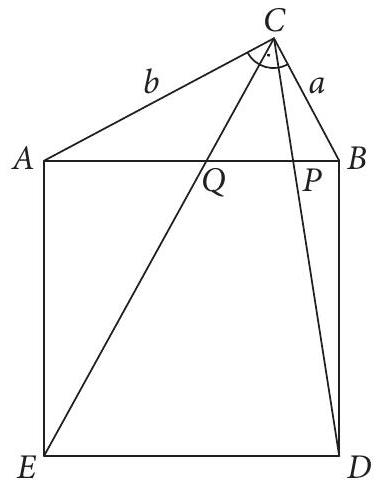
\includegraphics[max width=\textwidth, center]{2024_11_21_50d2fc5b1407ca7ef55bg-10}

Wykaż, że stosunek pola trapezu EDPQ do pola trójkąta QPC jest równy \(\left(\frac{1}{a}+\frac{1}{b}\right)^{2}\left(a^{2}+b^{2}\right)\).\\

\includegraphics[max width=\textwidth, center]{2024_11_21_50d2fc5b1407ca7ef55bg-10(1)}\\

\includegraphics[max width=\textwidth, center]{2024_11_21_50d2fc5b1407ca7ef55bg-11}

\begin{center}
\begin{tabular}{|l|l|c|}
\hline
\multirow{3}{*}{\begin{tabular}{c}
Wypełnia \\
sprawdzający \\
\end{tabular}} & Nr zadania & 11 \\
\cline { 2 - 3 }
 & Maks. liczba pkt & 3 \\
\cline { 2 - 3 }
 & Uzyskana liczba pkt &  \\
\hline
\end{tabular}
\end{center}

\section*{Zadanie 12. (0-4)}
Kąt przy wierzchołku \(A\) czworokąta \(A B C D\) jest prosty, a przekątna \(B D\) tego czworokąta jest prostopadła do boku \(B C\). W trójkąt \(A B D\) wpisano okrąg o środku \(O_{1}\) i promieniu 1, a w trójkąt \(B C D\) - okrąg o środku \(O_{2}\) i promieniu 2. Odcinek \(O_{1} O_{2}\) ma długość 3 (zobacz rysunek).\\
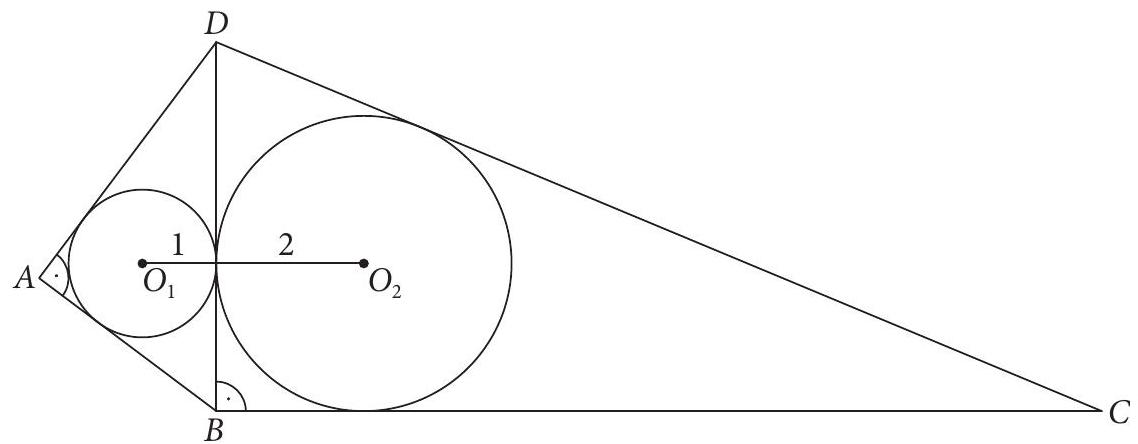
\includegraphics[max width=\textwidth, center]{2024_11_21_50d2fc5b1407ca7ef55bg-12}

Oblicz obwód czworokąta \(A B C D\).

\begin{center}
\begin{tabular}{|c|c|c|c|c|c|c|c|c|c|c|c|c|c|c|c|c|c|c|c|c|c|c|c|c|c|c|c|c|c|}
\hline
 &  &  &  &  &  &  &  &  &  &  &  &  &  &  &  &  &  &  &  &  &  &  &  &  &  &  &  &  &  \\
\hline
 &  &  &  &  &  &  &  &  &  &  &  &  &  &  &  &  &  &  &  &  &  &  &  &  &  &  &  &  &  \\
\hline
 &  &  &  &  &  &  &  &  &  &  &  &  &  &  &  &  &  &  &  &  &  &  &  &  &  &  &  &  &  \\
\hline
 &  &  &  &  &  &  &  &  &  &  &  &  &  &  &  &  &  &  &  &  &  &  &  &  &  &  &  &  &  \\
\hline
 &  &  &  &  &  &  &  &  &  &  &  &  &  &  &  &  &  &  &  &  &  &  &  &  &  &  &  &  &  \\
\hline
 &  &  &  &  &  &  &  &  &  &  &  &  &  &  &  &  &  &  &  &  &  &  &  &  &  &  &  &  &  \\
\hline
 &  &  &  &  &  &  &  &  &  &  &  &  &  &  &  &  &  &  &  &  &  &  &  &  &  &  &  &  &  \\
\hline
 &  &  &  &  &  &  &  &  &  &  &  &  &  &  &  &  &  &  &  &  &  &  &  &  &  &  &  &  &  \\
\hline
 &  &  &  &  &  &  &  &  &  &  &  &  &  &  &  &  &  &  &  &  &  &  &  &  &  &  &  &  &  \\
\hline
 &  &  &  &  &  &  &  &  &  &  &  &  &  &  &  &  &  &  &  &  &  &  &  &  &  &  &  &  &  \\
\hline
 &  &  &  &  &  &  &  &  &  &  &  &  &  &  &  &  &  &  &  &  &  &  &  &  &  &  &  &  &  \\
\hline
 &  &  &  &  &  &  &  &  &  &  &  &  &  &  &  &  &  &  &  &  &  &  &  &  &  &  &  &  &  \\
\hline
 &  &  &  &  &  &  &  &  &  &  &  &  &  &  &  &  &  &  &  &  &  &  &  &  &  &  &  &  &  \\
\hline
 &  &  &  &  &  &  &  &  &  &  &  &  &  &  &  &  &  &  &  &  &  &  &  &  &  &  &  &  &  \\
\hline
 &  &  &  &  &  &  &  &  &  &  &  &  &  &  &  &  &  &  &  &  &  &  &  &  &  &  &  &  &  \\
\hline
 &  &  &  &  &  &  &  &  &  &  &  &  &  &  &  &  &  &  &  &  &  &  &  &  &  &  &  &  &  \\
\hline
 &  &  &  &  &  &  &  &  &  &  &  &  &  &  &  &  &  &  &  &  &  &  &  &  &  &  &  &  &  \\
\hline
 &  &  &  &  &  &  &  &  &  &  &  &  &  &  &  &  &  &  &  &  &  &  &  &  &  &  &  &  &  \\
\hline
 &  &  &  &  &  &  &  &  &  &  &  &  &  &  &  &  &  &  &  &  &  &  &  &  &  &  &  &  &  \\
\hline
 &  &  &  &  &  &  &  &  &  &  &  &  &  &  &  &  &  &  &  &  &  &  &  &  &  &  &  &  &  \\
\hline
 &  &  &  &  &  &  &  &  &  &  &  &  &  &  &  &  &  &  &  &  &  &  &  &  &  &  &  &  &  \\
\hline
 &  &  &  &  &  &  &  &  &  &  &  &  &  &  &  &  &  &  &  &  &  &  &  &  &  &  &  &  &  \\
\hline
 &  &  &  &  &  &  &  &  &  &  &  &  &  &  &  &  &  &  &  &  &  &  &  &  &  &  &  &  &  \\
\hline
 &  &  &  &  &  &  &  &  &  &  &  &  &  &  &  &  &  &  &  &  &  &  &  &  &  &  &  &  &  \\
\hline
 &  &  &  &  &  &  &  &  &  &  &  &  &  &  &  &  &  &  &  &  &  &  &  &  &  &  &  &  &  \\
\hline
 &  &  &  &  &  &  &  &  &  &  &  &  &  &  &  &  &  &  &  &  &  &  &  &  &  &  &  &  &  \\
\hline
 &  &  &  &  &  &  &  &  &  &  &  &  &  &  &  &  &  &  &  &  &  &  &  &  &  &  &  &  &  \\
\hline
 &  &  &  &  &  &  &  &  &  &  &  &  &  &  &  &  &  &  &  &  &  &  &  &  &  &  &  &  &  \\
\hline
 &  &  &  &  &  &  &  &  &  &  &  &  &  &  &  &  &  &  &  &  &  &  &  &  &  &  &  &  &  \\
\hline
 &  &  &  &  &  &  &  &  &  &  &  &  &  &  &  &  &  &  &  &  &  &  &  &  &  &  &  &  &  \\
\hline
 &  &  &  &  &  &  &  &  &  &  &  &  &  &  &  &  &  &  &  &  &  &  &  &  &  &  &  &  &  \\
\hline
\end{tabular}
\end{center}

\begin{center}

\includegraphics[max width=\textwidth]{2024_11_21_50d2fc5b1407ca7ef55bg-13}
\end{center}

Odpowiedź:

\begin{center}
\begin{tabular}{|l|l|c|}
\hline
\multirow{2}{*}{\begin{tabular}{c}
Wypełnia \\
sprawdzający \\
\end{tabular}} & Nr zadania & 12 \\
\cline { 2 - 3 }
 & Maks. liczba pkt & 4 \\
\cline { 2 - 3 }
 & Uzyskana liczba pkt &  \\
\hline
\end{tabular}
\end{center}

Zadanie 13. (0-4)\\
Dany jest wielomian \(W(x)=-2 x^{3}+x+a^{2}\). Liczba \(a\) jest pierwiastkiem tego wielomianu, a reszta \(z\) dzielenia tego wielomianu przez dwumian \(2 x+a\) jest większa od \(a\). Oblicz \(a\).\\

\includegraphics[max width=\textwidth, center]{2024_11_21_50d2fc5b1407ca7ef55bg-14}\\

\includegraphics[max width=\textwidth, center]{2024_11_21_50d2fc5b1407ca7ef55bg-15}

Odpowiedź:

\begin{center}
\begin{tabular}{|l|l|c|}
\hline
\multirow{2}{*}{\begin{tabular}{c}
Wypełnia \\
sprawdzający \\
\end{tabular}} & Nr zadania & 13 \\
\cline { 2 - 3 }
 & Maks. liczba pkt & 4 \\
\cline { 2 - 3 }
 & Uzyskana liczba pkt &  \\
\hline
\end{tabular}
\end{center}

Zadanie 14. (0-6)\\
Wyznacz wszystkie wartości parametru \(m\), dla których przedział \((2,3)\) jest zawarty w zbiorze rozwiązań nierówności \((m+1) x^{2}+m x+1<0\).\\

\includegraphics[max width=\textwidth, center]{2024_11_21_50d2fc5b1407ca7ef55bg-16}\\

\includegraphics[max width=\textwidth, center]{2024_11_21_50d2fc5b1407ca7ef55bg-17}

Odpowiedź:

\begin{center}
\begin{tabular}{|l|l|c|}
\hline
\multirow{2}{*}{\begin{tabular}{c}
Wypełnia \\
sprawdzający \\
\end{tabular}} & Nr zadania & 14 \\
\cline { 2 - 3 }
 & Maks. liczba pkt & 6 \\
\cline { 2 - 3 }
 & Uzyskana liczba pkt &  \\
\hline
\end{tabular}
\end{center}

Zadanie 15. (0-6)\\
Punkt \(A=(-4,2)\) jest wierzchołkiem trójkąta równoramiennego \(A B C\). Punkt \(K=(2,0)\) leży na podstawie \(A B\) tego trójkąta, \(|A K|:|K B|=2: 1\). Punkt \(L=(0,6)\) leży na ramieniu \(A C\) tego trójkąta. Wyznacz współrzędne wierzchołków \(B\) i \(C\) oraz pole trójkąta \(A B C\).\\

\includegraphics[max width=\textwidth, center]{2024_11_21_50d2fc5b1407ca7ef55bg-18}\\

\includegraphics[max width=\textwidth, center]{2024_11_21_50d2fc5b1407ca7ef55bg-19}

Odpowiedź:

\begin{center}
\begin{tabular}{|l|l|c|}
\hline
\multirow{2}{*}{\begin{tabular}{c}
Wypełnia \\
sprawdzający \\
\end{tabular}} & Nr zadania & 15 \\
\cline { 2 - 3 }
 & Maks. liczba pkt & 6 \\
\cline { 2 - 3 }
 & Uzyskana liczba pkt &  \\
\hline
\end{tabular}
\end{center}

\section*{Zadanie 16. (0-7)}
Rozważmy wszystkie ostrosłupy prawidłowe trójkątne \(A B C S\), których suma długości wszystkich krawędzi jest równa 6. Podstawą ostrosłupa jest trójkąt \(A B C\).\\
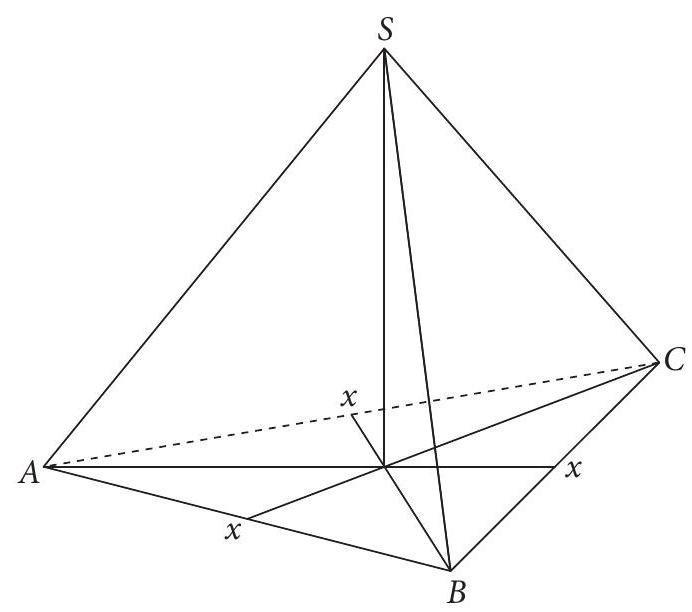
\includegraphics[max width=\textwidth, center]{2024_11_21_50d2fc5b1407ca7ef55bg-20}\\
a) Wykaż, że objętość \(V\) ostrosłupa, jako funkcja zmiennej \(x\) - długości krawędzi podstawy ostrosłupa, wyraża się wzorem \(V(x)=\frac{\sqrt{2}}{12} \cdot \sqrt{x^{6}-6 x^{5}+6 x^{4}}\). Dla jakich liczb rzeczywistych \(x\) liczba \(V(x)\) jest objętością tego ostrosłupa?\\
b) Wyznacz taką wartość \(x\), dla której funkcja \(V\) osiąga wartość największą. Oblicz tę największą wartość.

\begin{center}
\begin{tabular}{|c|c|c|c|c|c|c|c|c|c|c|c|c|c|c|c|c|c|c|c|c|c|c|c|c|c|c|c|c|c|}
\hline
 &  &  &  &  &  &  &  &  &  &  &  &  &  &  &  &  &  &  &  &  &  &  &  &  &  &  &  &  &  \\
\hline
 &  &  &  &  &  &  &  &  &  &  &  &  &  &  &  &  &  &  &  &  &  &  &  &  &  &  &  &  &  \\
\hline
 &  &  &  &  &  &  &  &  &  &  &  &  &  &  &  &  &  &  &  &  &  &  &  &  &  &  &  &  &  \\
\hline
 &  &  &  &  &  &  &  &  &  &  &  &  &  &  &  &  &  &  &  &  &  &  &  &  &  &  &  &  &  \\
\hline
 &  &  &  &  &  &  &  &  &  &  &  &  &  &  &  &  &  &  &  &  &  &  &  &  &  &  &  &  &  \\
\hline
 &  &  &  &  &  &  &  &  &  &  &  &  &  &  &  &  &  &  &  &  &  &  &  &  &  &  &  &  &  \\
\hline
 &  &  &  &  &  &  &  &  &  &  &  &  &  &  &  &  &  &  &  &  &  &  &  &  &  &  &  &  &  \\
\hline
 &  &  &  &  &  &  &  &  &  &  &  &  &  &  &  &  &  &  &  &  &  &  &  &  &  &  &  &  &  \\
\hline
 &  &  &  &  &  &  &  &  &  &  &  &  &  &  &  &  &  &  &  &  &  &  &  &  &  &  &  &  &  \\
\hline
 &  &  &  &  &  &  &  &  &  &  &  &  &  &  &  &  &  &  &  &  &  &  &  &  &  &  &  &  &  \\
\hline
 &  &  &  &  &  &  &  &  &  &  &  &  &  &  &  &  &  &  &  &  &  &  &  &  &  &  &  &  &  \\
\hline
 &  &  &  &  &  &  &  &  &  &  &  &  &  &  &  &  &  &  &  &  &  &  &  &  &  &  &  &  &  \\
\hline
 &  &  &  &  &  &  &  &  &  &  &  &  &  &  &  &  &  &  &  &  &  &  &  &  &  &  &  &  &  \\
\hline
 &  &  &  &  &  &  &  &  &  &  &  &  &  &  &  &  &  &  &  &  &  &  &  &  &  &  &  &  &  \\
\hline
 &  &  &  &  &  &  &  &  &  &  &  &  &  &  &  &  &  &  &  &  &  &  &  &  &  &  &  &  &  \\
\hline
 &  &  &  &  &  &  &  &  &  &  &  &  &  &  &  &  &  &  &  &  &  &  &  &  &  &  &  &  &  \\
\hline
 &  &  &  &  &  &  &  &  &  &  &  &  &  &  &  &  &  &  &  &  &  &  &  &  &  &  &  &  &  \\
\hline
 &  &  &  &  &  &  &  &  &  &  &  &  &  &  &  &  &  &  &  &  &  &  &  &  &  &  &  &  &  \\
\hline
 &  &  &  &  &  &  &  &  &  &  &  &  &  &  &  &  &  &  &  &  &  &  &  &  &  &  &  &  &  \\
\hline
 &  &  &  &  &  &  &  &  &  &  &  &  &  &  &  &  &  &  &  &  &  &  &  &  &  &  &  &  &  \\
\hline
 &  &  &  &  &  &  &  &  &  &  &  &  &  &  &  &  &  &  &  &  &  &  &  &  &  &  &  &  &  \\
\hline
 &  &  &  &  &  &  &  &  &  &  &  &  &  &  &  &  &  &  &  &  &  &  &  &  &  &  &  &  &  \\
\hline
 &  &  &  &  &  &  &  &  &  &  &  &  &  &  &  &  &  &  &  &  &  &  &  &  &  &  &  &  &  \\
\hline
 &  &  &  &  &  &  &  &  &  &  &  &  &  &  &  &  &  &  &  &  &  &  &  &  &  &  &  &  &  \\
\hline
 &  &  &  &  &  &  &  &  &  &  &  &  &  &  &  &  &  &  &  &  &  &  &  &  &  &  &  &  &  \\
\hline
\end{tabular}
\end{center}

\begin{center}

\includegraphics[max width=\textwidth]{2024_11_21_50d2fc5b1407ca7ef55bg-21}
\end{center}

Odpowiedź:

\begin{center}
\begin{tabular}{|l|l|c|}
\hline
\multirow{3}{*}{\begin{tabular}{c}
Wypełnia \\
sprawdzający \\
\end{tabular}} & Nr zadania & 16 \\
\cline { 2 - 3 }
 & Maks. liczba pkt & 7 \\
\cline { 2 - 3 }
 & Uzyskana liczba pkt &  \\
\hline
\end{tabular}
\end{center}

\section*{BRUDNOPIS (nie podlega ocenie)}
\begin{center}

\includegraphics[max width=\textwidth]{2024_11_21_50d2fc5b1407ca7ef55bg-22}
\end{center}


\end{document}